\documentclass[12pt,a4paper,pdftex]{article}

% Sprache
\usepackage[ngerman]{babel}
\usepackage[utf8]{inputenc}

\usepackage{graphicx}

% Page layout
\usepackage{geometry}
\geometry{a4paper,lmargin={2.5cm}, rmargin={2.5cm}, tmargin={2cm}, bmargin={2.5cm}}

% Figure and Caption layout
\usepackage[bf]{caption}
\usepackage{subcaption}
\usepackage{wrapfig}
\usepackage{setspace}

% Befehle zur Textauszeichnung (hervorheben, unterstreichen ect.)
\usepackage{color,soul}
\usepackage{xcolor} % bunter Text

% Zitier-Style für Bücher und URL
\usepackage[numbers]{natbib}
\usepackage[breaklinks=true,bookmarks=true,bookmarksopen=true,colorlinks=true,citecolor=black,linkcolor=black,urlcolor=gray,pdfpagemode=UseNone,pdfstartview=FitH]{hyperref}


\usepackage{float}
\usepackage{gensymb}
\usepackage{siunitx}
\usepackage{tabularx}
\usepackage{amsmath}

% für chemische zeichen
\usepackage[version=4]{mhchem}

% for commenting a whole section
\usepackage{verbatim}

\usepackage{pgfgantt}
\usepackage{afterpage}

% Index
\usepackage{imakeidx}
\makeindex[intoc, columnseprule]
\newcommand{\indextitle}{\section{Index}}

% Bilder importieren
\usepackage{epstopdf}
\epstopdfDeclareGraphicsRule{.pdf}{png}{.png}{convert #1 \OutputFile}
\DeclareGraphicsExtensions{.png,.pdf}

% Bildernummerierung fuer jedes kapitel
\usepackage{chngcntr}
\counterwithin{figure}{section}

% ich hab keine ahnung was die tun und wir brauchen sie auch nicht
%\newcommand{\command}[1]{\texttt{#1}}
%\newcommand{\fileextension}[1]{\texttt{#1}}

% plus minus zeichen
\newcommand{\rpm}{\raisebox{.2ex}{$\scriptstyle\pm$} }

% kapitel title auf deutsch
\renewcommand{\bibsection}{\section{Literaturverzeichnis}}



%%%%%%%%%%%%%%%%%%%%%%%%%%%%%%%%%%%%%%%%%%%%%%%%%%%%%%%%%%%%%

\begin{document}
\setlength{\parindent}{0pt}

%%%%%%%%%%%%%%%%%%%%%%%%%%%%%%%%%%%%%%%%%%%%%%%%%%%%%%%%%%%%%
% Titelseite
%%%%%%%%%%%%%%%%%%%%%%%%%%%%%%%%%%%%%%%%%%%%%%%%%%%%%%%%%%%%%

\begin{titlepage}
 \begin{center}
        \vspace*{1cm}
        \LARGE
        \textbf{Kurzes Lehrbuch der Neuroanatomie des Säugers}
        \vspace{2cm}
        
        \Large
        Praktikumsprotokoll des Mastermoduls Neuroanatomie
        \vspace{4cm}
        
        \large
        vorgelegt von \\ Jacqueline Göbl, Julia Grüb, Marta Provenzano und Laura Seidler % Author name
        \vfill
        \large     
        T\"ubingen, \today
    \end{center}
    \newpage
        \thispagestyle{empty}
        \mbox{}
        \newpage
\end{titlepage}


\thispagestyle{empty}
\mbox{}

%%%%%%%%%%%%%%%%%%%%%%%%%%%%%%%%%%%%%%%%%%%%%%%%%%%%%%%%%%%%%% Inhaltsverzeichnis und Abbildungsverzeichnis
%%%%%%%%%%%%%%%%%%%%%%%%%%%%%%%%%%%%%%%%%%%%%%%%%%%%%%%%%%%%%

\tableofcontents
\newpage
\listoffigures

%%%%%%%%%%%%%%%%%%%%%%%%%%%%%%%%%%%%%%%%%%%%%%%%%%%%%%%%%%%%%
% Textbeginn
%%%%%%%%%%%%%%%%%%%%%%%%%%%%%%%%%%%%%%%%%%%%%%%%%%%%%%%%%%%%%
\newpage

\subsection{Beschriftung und Kürzel}
%%%%%%%%%%%%%%%%%%%%%%%%%%%%%%%%%%%%%%%%%%%%%%%%%%%%%%%

\begin{comment}
2n \indent - \indent \textit{N. opticus}\\
3V \indent - \indent Dritter Ventrikel\\
3n \indent - \indent \textit{N. oculomotorius}\\
4V \indent - \indent Vierter Ventrikel\\
ACx \indent - \indent Archicortex\\
Aq \indent - \indent Aquädukt, \textit{Aqueductus mesencephali, Aquaeductus cerebri}\\
Cb \indent - \indent Cerebellum, Kleinhirn\\
cc \indent - \indent \textit{Corpus callosum}\\
CCx \indent - \indent cingulärer Cortex, \textit{Gyrus cinguli}\\
ce \indent - \indent \textit{Capsula externa}\\
Chp \indent - \indent \textit{Choroid plexus}\\
cp \indent - \indent Kleinhirn-Pedunkel\\
CPu \indent - \indent Caudoputamen\\
CS\indent - \indent Rückenmark\\
Cu \indent - \indent \textit{Nucleus caudatus}\\
Cx \indent - \indent cerebraler Cortex, \textit{Cortex cerebri}\\
Epi \indent - \indent Epiphyse\\
f \indent - \indent Fornix\\
fi \indent - \indent Fimbria\\
Hip \indent - \indent Hippocampus\\
IC \indent - \indent \textit{Colliculus inferior}\\
LGN \indent - \indent \textit{Corpus geniculatum laterale}\\
LV \indent - \indent lateraler Ventrikel\\
MB \indent - \indent Mammillarkörper\\
Med \indent - \indent Medulla, \textit{Medulla oblongata}\\
NCx \indent - \indent Neocortex\\
OB \indent - \indent \textit{Bulbus olfactorius}\\
ox \indent - \indent optisches Chiasma, \textit{Chiasma opticum}\\
PM \indent - \indent Pia mater\\
Pon \indent - \indent Pons\\
RF \indent - \indent \textit{Fissura rhinalis}\\
SA \indent - \indent \textit{Sulcus ansatus}\\
SC \indent - \indent \textit{Colliculus superior}\\
TC \indent - \indent Hirnstamm, \textit{Truncus cerebri, Truncus encephali}\\
Teg\indent - \indent Tegmentum, \textit{Tegmentum mesencephali}\\
Th \indent - \indent Thalamus\\
tz \indent - \indent Trapezkörper\\
ve \indent - \indent Velum\\
\end{comment}

\begin{table}[H]
\begin{tabular}{llcll}
           & 3V  & \textbf{-} & Dritter Ventrikel                                                       & \multicolumn{1}{c}{\textbf{}} \\
\textbf{}  & 3n  & -          & N. oculomotorius                                                        & \multicolumn{1}{c}{}          \\
\textbf{}  & 4V  & -          & Vierter Ventrikel                                                       & \multicolumn{1}{c}{}          \\
\textbf{A} & ACx & -          & Archicortex                                                             & \multicolumn{1}{c}{}          \\
\textbf{}  & Aq  & -          & Aquädukt, Aqueductus mesencephali, Aquaeductus cerebri                  & \multicolumn{1}{c}{}          \\
\textbf{C} & Cb  & \textbf{-} & Cerebellum, Kleinhirn                                                   & \multicolumn{1}{c}{\textbf{}} \\
           & cc  & \textbf{-} & Corpus callosum                                                         & \multicolumn{1}{c}{\textbf{}} \\
\textbf{}  & CCx & -          & cingulärer Cortex, Gyrus cinguli             & \multicolumn{1}{c}{}          \\
\textbf{}  & ce  & -          & Capsula externa                                                         & \multicolumn{1}{c}{}          \\
\textbf{}  & Chp & -          & Choroid plexus                                                          & \multicolumn{1}{c}{}          \\
\textbf{}  & cp  & -          & Kleinhirn-Pedunkel                                                      & \multicolumn{1}{c}{}          \\
\textbf{}  & CPu & -          & Caudoputamen                                                            &                               \\
\textbf{}  & CS  & -          & Rückenmark                                                              &                               \\
\textbf{}  & Cu  & -          & Nucleus caudatus                                                        &                               \\
\textbf{}  & Cx  & -          & cerebraler Cortex, Cortex cerebri          &                               \\
\textbf{E} & Epi & -          & Epiphyse                                                                &                               \\
\textbf{F} & f   & -          & Fornix                                                                  &                               \\
\textbf{}  & fi  & -          & Fimbria                                                                 &                               \\
\textbf{H} & Hip & -          & Hippocampus                                                             &                               \\
\textbf{I} & IC  & -          & Colliculus inferior                                                     &                               \\
\textbf{L} & LGN & -          & Corpus geniculatum laterale                                             &                               \\
\textbf{}  & LV  & -          & lateraler Ventrikel                                                     &                               \\
\textbf{M} & MB  & -          & Mammillarkörper                                                         &                               \\
\textbf{}  & Med & -          & Medulla, Medulla oblongata                  &                               \\
\textbf{N} & NCx & -          & Neocortex                                                               &                               \\
\textbf{O} & OB  & -          & Riechkolben, Bulbus olfactorius                                                      &                               \\
\textbf{}  & ox  & -          & optisches Chiasma, Chiasma opticum           &                               \\
\textbf{P} & PM  & -          & Pia mater                                                               &                               \\
\textbf{}  & Pon & -          & Pons                                                                    &                               \\
\textbf{R} & RF  & -          & Fissura rhinalis                                                        &                               \\
\textbf{S} & SA  & -          & Sulcus ansatus                                                          &                               \\
\textbf{}  & SC  & -          & Colliculus superior                                                     &                               \\
\textbf{T} & TC  & -          & Hirnstamm, Truncus cerebri, Truncus encephali &                               \\
\textbf{}  & Teg & -          & Tegmentum, Tegmentum mesencephali           &                               \\
\textbf{}  & Th  & -          & Thalamus                                                                &                               \\
\textbf{}  & tz  & -          & Trapezkörper                                                            &                               \\
\textbf{V} & ve  & -          & Velum                                                                   &                              
\end{tabular}
\end{table}
%%%%%%%%%%%%%%%%%%%%%%%%%%%%%%%%%%%%%%%%%%%%%%%%%%%%%%%%%%%
%%%%%%%%%%%%%%%%%%%%%%%%%%%%%%%%%%%%%%%%%%%%%%%%%%%%%%%%%%%

\newpage
\section{Spezielle sensorische Bahnen}
% verweis auf dieses Kapitel mit \ref{sec:spezsens}
\label{sec:spezsens}
Die speziellen sensorischen Bahnen umfassen unter anderem die Hörbahn, die Sehbahn und die Riechbahn, womit sich in diesem Kapitel vor allem beschäftigen wird. Diese drei speziellen sensorischen Bahnen spielen sowohl bei der Ratte als auch beim Schaf die zentrale Rolle. Es gibt weiter spezialisierte Sinne wie zum Beispiel den elektrischen Sinn bei Fischen, die beiden chemischen Sinne für Geruch und Geschmack und der Magnetsinn bei Zugvögeln \textsuperscript{\cite{smith2008biology}}. Diese werden nicht in dieser Zusammenfassung behandelt, spielen aber bei anderen Tierarten eine tragende Rolle und sollten aus diesem Grund hier kurz erwähnt werden.

\subsection{Hörbahn}

Das auditorische System ist für die Verarbeitung von Schallwellen, die über die Luft oder Wasser übertragen und vom System empfangen werden, zuständig. Vibrationen die über den Untergrund oder festes Substrat übertragen werden und mechanisch wahrgenommen werden, gehören zum Vibrationssinn der eng verwandt mit dem auditorischen Sinn ist.
\\
\noindent Dabei hat der auditorische Sinn zwei Aufgaben: zum einen die Detektion des Schalls und die Lokalisation der Schallwelle. Das Richtungshören ist nicht für alle Tiere möglich und ist auch bei den Tieren die dazu befähigt sind, nicht im gesamten Hörbereich gleich genau \textsuperscript{\cite[18]{penzlin2005tierphys}}.

\subsubsection*{Spiralganglion}
Die Funktion unserer Ohren ist die Energie eines akustischen Signals von der Außenwelt einzufangen und von einem mechanischen Signal in ein elektrisches Signal umzuwandeln. Diese Umwandlung findet an den inneren Haarsinneszellen in der Cochlea statt. Dort wird durch die Auslenkung der Haarbündel an den inneren Haarsinneszellen (eng.: inner hair cell, IHC) die Zelle depolarisiert oder hyperpolarisiert je nach Auslenkungsrichtung \textsuperscript{\cite[30]{kandel2013principles}}. Die Depolarisation der Haarzellen führt zur Öffnung spannungsgesteuerter Kalziumkanäle und dem damit verbundenen Einstrom von \ce{Ca^2+}. Durch den Einstrom des \ce{Ca^2+} wird der Neurotransmitter (wahrscheinlich Glutamat) freigesetzt und aktiviert die Spiralganglionzelle. \textbf{Spiralganglionzellen} sind bipolare Zellen, welche ihren Namen der spiralförmigen Struktur der Cochlea (Schneckenspindel) verdanken, der sie folgen\textsuperscript{\cite[11]{neurowissenschaften_baer}}. Sie formen einen Teil des achten Hirnnervs (CN~VIII), der auch \textbf{Nervus vestibulocochlearis} genannt wird. Ungefähr 30~000 Ganglionzellen im Hörnerv werden durch die inneren Haarzellen innerviert, das macht ungefähr 90\% des Nervs aus\textsuperscript{\cite[30]{kandel2013principles}}. 
Innere Haarzellen haben keinen efferente Eingang von höheren Hirnstrukturen. Anhand der Neuronenverteilung in der afferente Bahn wird die funktionale Bedeutung zwischen den inneren und äußeren Haarzellen erkennbar. Die afferenten Fasern ausgehend von den IHC sind myelinisiert (Typ I) und bilden 95\% der affrenten Fasern, wärend 5\% der Fasern, affrente unmyelinsierte Typ~II Fasern, von den äußeren Haarzellen kommen. Bei den inneren Haarzellen gibt dabei die Regel: Jedes Axon wird nur von eine Haarzelle innerviert, aber eine Haarzelle innerviert im Durchschnitt zehn Fasern.  \textsuperscript{\cite[30]{kandel2013principles}}.   
\\
\noindent Die affrenten Nervenfasern der IHC codieren die Stimulusfrequenz und die Intensität. Auf Grund der Beschaffenheit der Basilarmembran der Cochlea, werden die Frequenzen tonotopisch von hohen Frequenzen am ovalen Frenster bis zu tiefen Tönen am Helicotrema an der Basilarmembran entlang aufgeteilt\textsuperscript{\cite[29]{paxinos2014rat}}. Aufgrund ihrer Größe und Funktion sind die Type I Fasern, ausgehend von den inneren Haarzellen, sehr viel besser verstanden. Die Bahnen die die Informationen aus diesen Fasern nehmen werden im Folgenden als einzige thematisiert.

\begin{figure}[H]
    \centering
    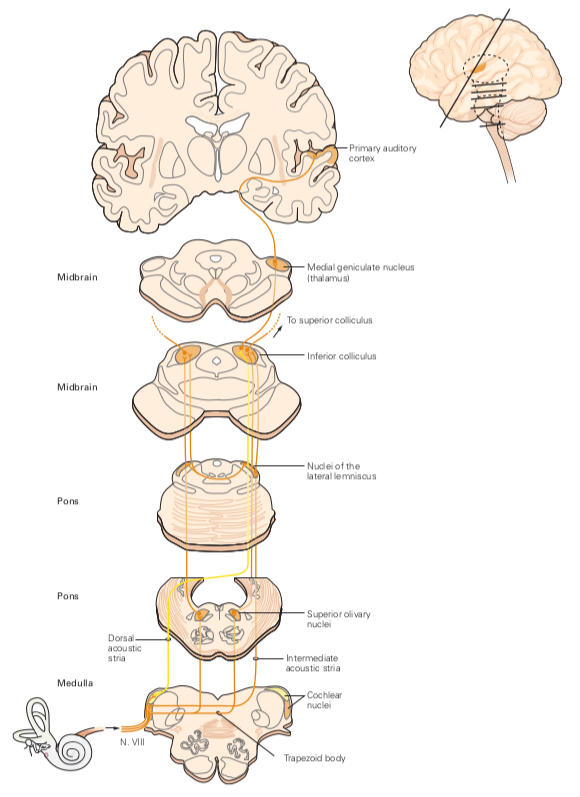
\includegraphics{pictures/auditory/hoerbahn_pathway.png}
    \caption[Hörbahn]{\textbf{Hörbahn} \\
    Die einzelnen Stationen der Hörbahn des Menschen von den Spiralganglionzellen in der Cochlea bis zum primären auditorischen Cortex anhand skizzierter Gehirnschnitte aus dem Kandel\textsuperscript{\cite[30]{kandel2013principles}} und einem Fließdiagramm}
    \label{fig:hoerbahn_pathway}
\end{figure}

\newpage
\noindent Efferente Fasern im Hörnerv innervieren die äußeren Haarzellen in der Cochlea, deren Aufgabe darin besteht die mechanische Auslenkung der Basilarmembran und der damit verbundenen Tektorialmembran zu verstärken oder zu unterdrücken. Infolgedessen kommt es zu einer verstärkten Selektivität und Sensibilität der Frequenzwahrnehmung\textsuperscript{\cite[29]{paxinos2014rat}}.

\subsubsection*{Nucleus cochlearis}

Die afferenten Ganglionzellen aus dem Hörnerv ziehen auf der Höhe der Medulla in den Hirnstamm und dort in das Kerngebiet den \textbf{Nucleus cochlearis} (\textbf{CN}). Dieser befindet sich  lateral auf der Höhe der Medulla (Abb.~\ref{fig:hoerbahn_pathway}) und bekommt nur Input aus dem Hörnerv der ipsilateralen Seite. Der NC besteht aus dem dorsalen Nucleus cochlearis (DCN) und dem ventralen Nucleus cochlearis (VCN), welcher wiederum in den anteroventralen (AVCN) und den posteroventralen (PVCN) Nucleus unterteilt wird\textsuperscript{\cite[29]{paxinos2014rat}}. Bei Ratten liegt der ventrale Nucleus cochlearis flach mediolateral an der Medulla, während der dorsale Nucleus cochlearis sich um den 'restiform body'\textsuperscript{\cite[29]{paxinos2014rat}}.
\\ \noindent Die auditorischen Nervenfasern verzweigen sich im Nucleus cochlearis in die verschiedenen Teile des CNs (Abb.~\ref{fig:Nucleus_cochlearis}B). Jede Faser gabelt sich in einen aufsteigen Ast zum AVCN und einen absteigenden Ast zum PVCN und DCN und leitet die Informationen an verschiedene Neurone in den Teilbereichen weiter\textsuperscript{\cite[29]{paxinos2014rat}}. Die Neuronen im ventralen Nucleus cochlearis codieren verschieden Eigenschaften, je nach Zelltyp. Im Allgemeinen schärfen sie das Timing und die Information aus dem Klangspektrum. 
\\

\begin{figure}[H]
    \centering
    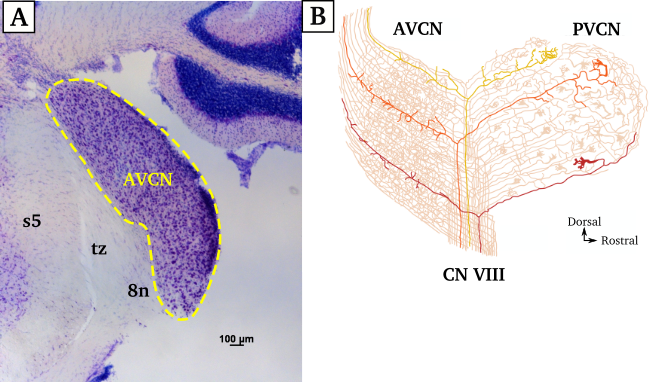
\includegraphics[width = \textwidth]{pictures/auditory/CN.png}
    \caption[Nucleus cochlearis]{\textbf{Nucleus cochlearis}\\
    \textbf{A}: Nissel-Färbung (N09\_1DL) der rechten Seite der Medulla. Es sind der anteroventrale Nucleus cochlearis (AVCN), der Trigeminus (s5), der Trapezkörper (tz) und der achte Hirnnerv (8n, Hörnerv) zu sehen. \textbf{B}: Verlauf der Nervenfasern aus dem achten Hirnnerv (CN VIII, 8n) im ventralen Nucleus cochlearis. Sowohl im anteroventralen (AVCN) als auch im posteroventralen (PVCN) Bereich des CNs werden die Fasern nach der Frequenz tonotopisch geordnet, von den tiefen Frequenzen (rot) ventral bis zu den hohen Frequenzen (gelb) im dorsalen Bereich. Abbildung B verändert nach Kandel \textsuperscript{\cite[31]{kandel2013principles}}}
    \label{fig:Nucleus_cochlearis}
\end{figure}

\newpage
Ein wesentlichen Teil spielt das Timing in der Weiterverarbeitung der Informationen in der oberen Olive, wohingegen die Verarbeitung des Klangspektrums in den ipsilateralen DCN, die ipsilaterale laterale obere Olive (LSO), den contralateralen ventralen Nucleus des lateralen Lemniscus und den contraleteralen Colliculus inferior projiziert wird. Ein Teilder Neuronen des Nucleus cochlearis projiziert in den contralateralen oberen paraoliven Nucleus (SPO) und den ventralen Nucleus des lateralen Lemniscus (VLL). Man nimmt an dass diese Bahnen bei der Verarbeitung von Störsignalen und Periodizität, sowie der Erkennung von Tonmustern eine Rolle spielt\textsuperscript{\cite[31]{kandel2013principles}}.  
\\\\
\noindent Der dorsale Nucleus cochlearis bekommt einerseits direkten Input von den Neuronen aus dem Hörnerv, zum anderen indirekten Input aus dem ventralen CN. Der dorsale CN integriert akustische  und somatosensorische Informationen um die Richtung der Schallquelle zu bestimmen\textsuperscript{\cite[31]{kandel2013principles}}.


\subsubsection*{Obere Olive}
Ein Großteil der Nervenzellen aus dem Nucleus cochlearis projizieren in die obere Olive. Die \textbf{obere Olive} (\textit{Nucleus olivaris superior}) ist für die Verarbeitung auditorischer Informationen wichtig und umfasst mehrere Kerngebiete. Innerhalb der Säugetiere variieren die Kerngebiete die unter dem Begriff obere Olive zusammengefasst werden. Drei Kerngebiete können bei fast allen Spezies gefunden werden: die \textbf{laterale obere Olive} (eng.: lateral superior olive, \textbf{LSO}), die \textbf{mediale obere Olive} (eng.: medial superior olive, \textbf{MSO}) und der \textbf{mediale Nucleus des Trapezkörpers} (eng.: medial nucleus of the trapezoid body, \textbf{MNTB}). Die LSO ist ein S-förmiges Kerngebiet im lateralen bereich der oberen Olive und ist durch ihre markante Struktur leicht zu erkennen (Abb.~\ref{fig:obere_Olive}). Die MSO liegt medial der LSO und ist bei Ratten ein kleineres Kerngebiet als beim Menschen. Der mediale Nucleus des Trapezkörpers (MNTB) befindet sich lateral in der oberen Olive\textsuperscript{\cite[29]{paxinos2014rat}}.

In Nagetieren, wie der Ratte, gibt es ein viertes, ausgeprägtes Kerngebiet, den \textbf{oberen paraoliven Nucleus} (eng.: superior paraolivary nucleus, \textbf{SPO}). Diese Kerngebiet befindet sich im dorsomedial Bereich der oberen Olive. Es bekommt die Informationen aus dem contralateralen Nucleus cochlearis und projiziert in den Colliculus inferior auf der ipsilateralen Seite\textsuperscript{\cite[29]{paxinos2014rat}}.
\\\\
\noindent Die drei Hauptkerne der oberen Olive spielen eine wichtige Rolle in der Verarbeitung von Schall. Aufgrund der Beschaffenheit der Cochlea werden dort nur die einzelnen Frequenzen kodiert, wobei dadurch keine Informationen über die Richtung der Schallquelle kodiert werden. Das Richtungshören wird in der oberen Olive integriert, durch die Verarbeitung der Informationen aus beiden Ohren. Sie ist damit die erste Schaltstelle in der Hörbahn die Input von der ipsilateralen und der contralateralen Seite, aus den jeweiligen Nuclei cochearis, bekommt.

Die mediale obere Olive (\textbf{MSO}) verarbeitet vorrangig tiefe Töne und berechnet, über das '\textit{phase-locking}' die Zeitdifferenz der beiden Phasen, die Richtung aus der der Ton kam. 
\textcolor{red}{MSO - Input\\     - Funktion\\     - Projektion\\ LSO und MNTB  - Input\\     - Funktion\\     - Projektion}

\begin{figure}[H]
    \centering
    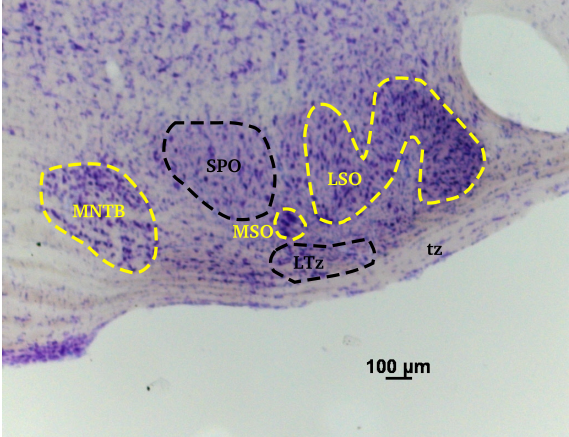
\includegraphics{pictures/auditory/obere_olive.png}
    \caption[Obere Olive]{\textbf{Obere Olive}\\
    Nissel-Färbung (N10\_1DL) der oberen Olive in der Pons. Mit den drei Hauptkernen mediale obere Olive (MSO), der lateralen oberen Olive (LSO) und dem medialen Nucleus des Trapezkörpers (MNTB) und dem für Nager speziellen oberen paraoliven Nucleus (SPO). Des weiteren liegt in der oberen Olive das Kerngebiet des lateralen Nucleus des Trapezkörpers (LTz) und der Trapezkörper (tz) selber, welcher die oberen Oliven beider Hirnhälften miteinander verbindet, befindet sich ventral des Komplex der oberen Olive.}
    \label{fig:obere_Olive}
\end{figure}

\begin{itemize}
    \item function: binaurale verschaltung integration von beiden ohren führt zu richtungs hören
    \item laterale obere olive und mntb für Interaurale intensitäts diffrenz
    \item mediale obere olive für interaurale zeit diffrenz ( tiefe töne) warum bei ratten nochmal kleiner???
    \item ohrenabstand für interaurale zeitdiffrenz zu klein desswegen wenig über medilae olive
    \item wo gehen die zellen dann genau hin
\end{itemize}


\subsubsection*{Lateraler Lemniscus}

\begin{figure}
    \centering
    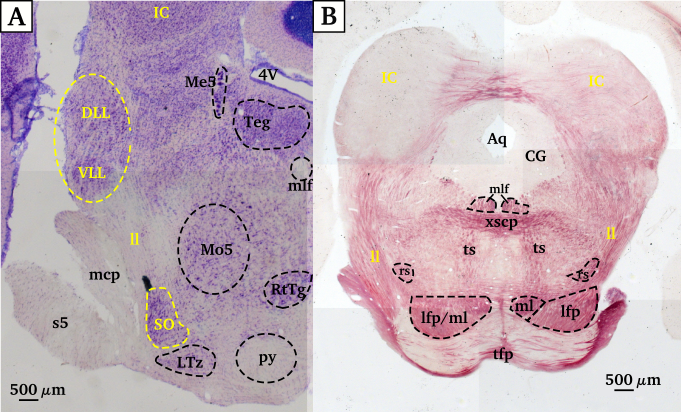
\includegraphics{pictures/auditory/lateral_lemniscus.png}
    \caption[Lateraler Lemniscus und seine Kerne]{\textbf{Lateraler Lemniscus und seine Kerne}\\
    }
    \label{fig:lateraler_lemniscus}
\end{figure}


    \begin{itemize}
        \item nerven aus der oberen olive ziehen durch den nervenstrang der lateraler leminiscus heißt in den inferior colliculus aber manche sind nochmal zwischen geschaltet in den kernen des lateralen leminiscus ( gibts da ihrgend eine regel oder aufteilung welche verschaltet sind und welche nicht??)
        \item was ist dann der grund für die verschaltung und welche funktion hat der laterale leminiscus -ausser transport ????
    \end{itemize}


\subsubsection*{Colliculus inferior}

    \begin{itemize}
        \item 
    \end{itemize}

\subsubsection*{Nucleus geniculatum mediale}

\subsubsection*{Primärer auditorischer Cortex}

\newpage
\subsection{Sehbahn}
\begin{itemize}
    \item eye
    \begin{itemize}
        \item kurzer überblick über die entwicklung des auges in der embryonal entwicklung retina aus dem diencephalon
        \item auf grund der evolutionären Entwicklunf ein "inverted" auge wesswegen die retina und die photorezeptoren nach innen weg vom licht gerichtet sind
        \item formung der retina: \cite{smith2008biology} p.287
        \item retinale zellen Stäbchen und zäpfchen und dann bipolar zellen und Ganglienzellen 
        \item vllt was zu den rezeptifen feldern
    \end{itemize}
    \item visual pathway
    \begin{itemize}
        \item 3 verschiedene wege ( vorlesung von oswald IN)
        \item wie heißen die von führen sie hin und wir konzentrieren uns auf einen zentralen und warum
    \end{itemize}
    \item optic nerve von der Retina zum Chiasma opticum
    \item Optic chiasm    \index{Optic chiasm}
    \begin{itemize}
        \item Semidecussation  \index{Decussation!Semi-}
        \item ganglienzellen von der nasalen/medialen seite des auges kreuzen am optic chiasm auf die andere seite des gehirns wärend die laterale seite des auges auf der selben seite weiter projezieren
        ßitem keine verschaltung im optischen chiasma sondern nur eine kreuzung der ganglien zellen
        \item danach optic tract
    \end{itemize}
    \item Optic tract \index{Optic tract}
    \item LGN: nicht gestreift, hinterer Teil das Thalamus \index{Thalamus}, auf Höhe des superior colliculus \index{SC!Superior culliculus}
    \begin{itemize}
        \item lateral am Diencephalon \index{Diencephalon} vorbei
        \item posteriorer part des thalamus
        \item aufbau des LGN unterschied zwischen primaten (6 Schichten) und Ratten bzw. Schafen
        \item kurz was zur funktion der verschaltung auf der ebene ( vllt etwas zu den rezeptive fields aber dann auch schon auf der ebene der retina erwähnen)
        \item von LGN über die optic radiation (welche nicht in den schnitten sichtbar ist) ruaf in den neocortex und in V1 
    \end{itemize}
    \item Magnifikationsfaktor = Dichte der Zellen und wie sie verschaltet sind
    \\
\end{itemize}
\subsection{(Riechbahn)}
\begin{itemize}
    \item vom olfactorischen bulb über den olfactorischen trakt zu einerm der ältesten teile des neocortex zum Pyriformen lappen
    \item weitere neuronen führen dann zum thalamus un die weitern stränge dann in den orbitofrontal lobe \cite{smith2008biology} 
    \item eventuell Dopaminerge Bilder
\end{itemize}

%%%%%%%%%%%%%%%%%%%%%%%%%%%%%%%%%%%%%%%%%%%%%%%%%%%%%%%%%%5%%
% Bibliography

\newpage
\bibliographystyle{unsrt}
\bibliography{references}

%%%%%%%%%%%%%%%%%%%%%%%%%%%%%%%%%%%%%%%%%%%%%%%%%%%%%%%%%%%%%
% Index
\printindex

2n - II optic nerve
3V - 3. Ventrikel\\
3n - III oculomotor nerve\\
4V - 4. Ventrikel\\
5n - V Trigeminus\\
6n - VI nervus abducens\\
\\
Aq - Aquaeductus cerebri\\
Amy - Amygdala\\
ACx - Archicortex\\
\\
CCx - cingulärer Cortex\\
Cu - Nucleus caudatus\\
CPu - Caudoputamen (Striatum)\\
cc - corpus callosum / Balken\\
ChP - choroid plexus\\
Cx - cerebraler Cortex\\
cp - cerebellar peduncle\\
CS - cortical Spine / cortikales Rückenmark\\
Cb - Cerebellum\\
\\
Epi - Epiphyse\\
EO - epithelium olfactorium\\
\\
f - Fornix\\
fi - Fimbria\\
\\
Hi - Hippocampus\\
Hyp - Hypophyse\\
\\
IC - Inferior colliculus\\
ICj - Islands of Calleja\\
\\
LGN - lat. genuculate nuc.\\
lot - lat. olfactory tract\\
LV - lateraler Ventrikel
\\
Med - Medulla\\
MB - mammillary body\\
\\
NCx - Neocortex\\
\\
OB - olfactory bulb / Riechkolben\\
ox - chiasma opticum\\
ot - olfactory tract / olfaktorischer Trakt\\
\\
Pon - Pons\\
PM - Pia mater\\
\\
RF - rhinal fissure\\
\\
SC - Superior colliculus / Colliculus inferior\\
\\
Th - Thalamus\\
Teg - Tegmentum\\
tz - trapezoid body / Trapezkörper\\
TC - Truncus cerebri / Hirnstamm\\
Tu - olfactory tubercle\\
\\
Ve - Velum\\
\\



\end{document}


